\documentclass[main.tex]{subfiles}
\begin{document}
	
	\chapter{Planning}
		\chapterauthor{\todo{add Author}}
	
	 The Planning team consisting of Jan Schimpf (Groupleader), Philipp Klein (Manipulation), Tom-Eric Lehmkuhl (Knowledge) and Torge Olliges (Perception) was basically responsible for the integration and connection of the results of the other groups. To achieve this task the planning group orientated itself along the lines of the legacy code of our predecessors and came up with the general architecture of the project. The planning grou was also mainly in charge of testing on the HSR. At the beginning we choose a project/directory structure which fitted our needs and splitted the tasks so that every group had a specific person who was responsible for them as declared above. During the time that we worked on milestone 1 we communicated our progress and current tasks in the group so that everybody knew what the other group members are doing and how we were progressing. In the following sections we will explain the concrete tasks and provide results of our work.

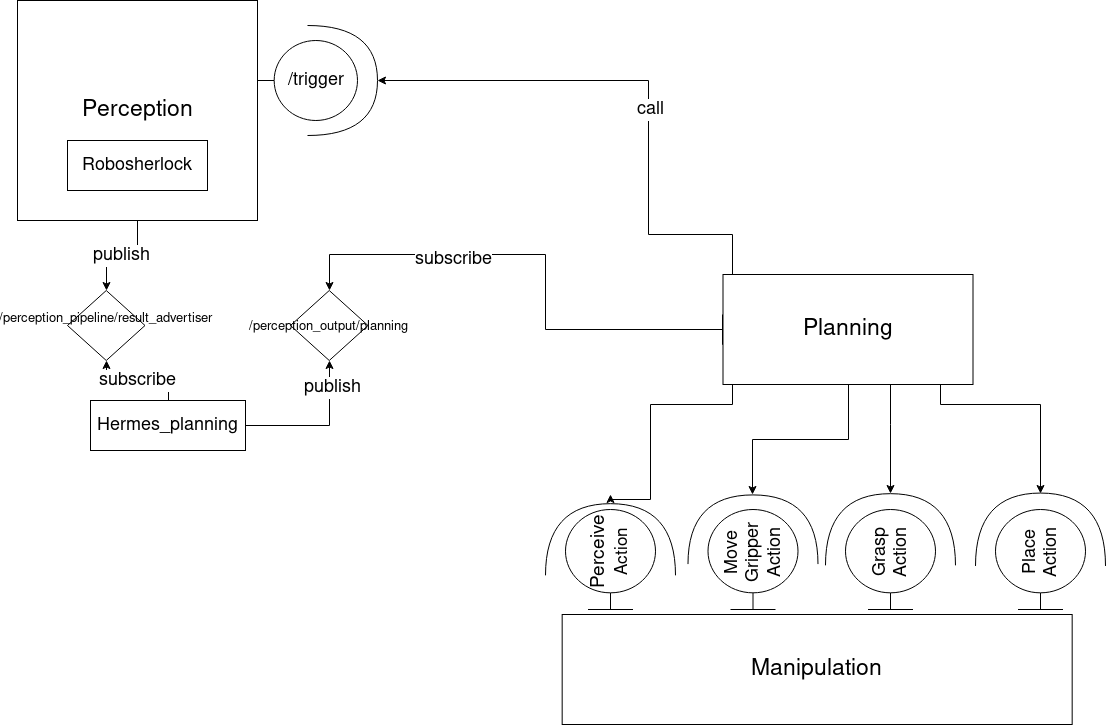
\includegraphics[scale=0.5]{subdocuments/architecture.png}

\section{Manipulation}

                The main task for the manipulation part of planning was to implement four action clients which are used to communicate with the action servers of the manipulation group.
		\begin{lstlisting}
                1. Move gripper client
                2. Place action client
                3. Perceive action client
                4. Grasp action client
		\end{lstlisting}

		\subsection{Move gripper client}

		The move gripper client is responsible for starting the arm movement. A target position is defined and encapsulated as a geometry\_msgs/PoseStamped message that will be passed to the manipulation action server via the manipulation/MoveGripperAction topic which executes the movement. Afterwards it is returned whether the message was successfuly created and published. 

		\subsection{Place action client}

    The place action client is responsible for starting the movement of an object in the gripper to a target position. The position is set and published to the action server as geometry\_msgs/PosedStamped message via the manipulation/PlaceAction topic. It returns whether the message was successfully created and published.

    \subsection{Perceive action client}

		The perceive action server is responsible for initiating the taking of a pose for perceiving an object. A distinction is made between three poses, which are coded as int: 
		\begin{lstlisting}
      perceive_arm_low = 0
      percieve_side = 1
      perceive_arm_high = 2
		\end{lstlisting}
Additionally the torso-joint-state is passed as float.
The whole thing is published as a message about the manipulation/PerceiveAction topic to the manipulation action server. Afterwards it is returned whether the message was successfuly created and published.

		\subsection{Grasp action client}

		The grasp action client is responsible for starting the gripping of an object. The object is identified by the object\_frame\_id, which is published as a string message via the Manipulation/GrapsAction topic to the action server of Manipulation. Afterwards it is returned whether the message was successfuly created and published.

		\section{Perception}

		The main task for the perception part of the planning group was to implement a client which triggers the perception pipeline.
		The first implementation was a simple node which tried to establish a connection to the perception pipeline trigger service and send a trigger request so that the perception pipeline would start running and processing the input. But this was later changed due to the fact that we couldn't know if the perception pipeline did it's job properly.
		So we implemented a action client which is similar to the client which was used by our predecessors because the perception group also implemented a action server which is similar to the legacy code. With the new action server and client we can now receive a success message from the perception server if the pipeline completed successfully.

		\section{Navigation}

                The main task for the navigation part of the planning group was to implement an action client which connects to the navigation groups action server.

		\section{Knowledge}

                The group member which was responsible for the knowledge part of the planning group couldn't achieve it's initial goal due to the fact that we never receiver a proper description of the knowledge group on how to communicate with their nodes. Thus the group member was used to support the manipulation part of planning.


\end{document}
